\section{Comparaci\'on entre todos los m\'etodos}

Una vez elegidos los mejores valores de configuracion para cada heurıstica implementada (si fue posible), realizar una experimentacion sobre un conjunto nuevo de instancias para observar la performance
de los metodos comparando nuevamente la calidad de las soluciones obtenidas y los tiempos de ejecucion en funcion de los parametros de la entrada. 
Para los casos que sea posible, comparar tambien los resultados del algoritmo exacto implementado.
Presentar todos los resultados obtenidos mediante graficos adecuados y discutir al respecto de los mismos.
\subsection{Resultados}
\subsubsection{Nodos fijos}
Aqu\'i se comparan los resultados de los 3 algoritmos (Grasp, Greedy y Local), manteniendo los nodos fijos. Nuestros tests fueron con nodos fijos desde 100 hasta 1000 y para cada una de esas instancias,
variando los ejes de a 100, comenzando con 1000 ejes.\\

En estos gr\'aficos, vamos a buscar, para cada cambio en los ejes, cu\'al fue el que menos nodos utiliza en su respuesta. \'Este ser\'a el mejor en cuanto a resultados.\\

Mostraremos los gr\'aficos con 100, 300, 600 y 900 nodos fijos:

 \begin{figure}[h!]
   \begin{center}
 	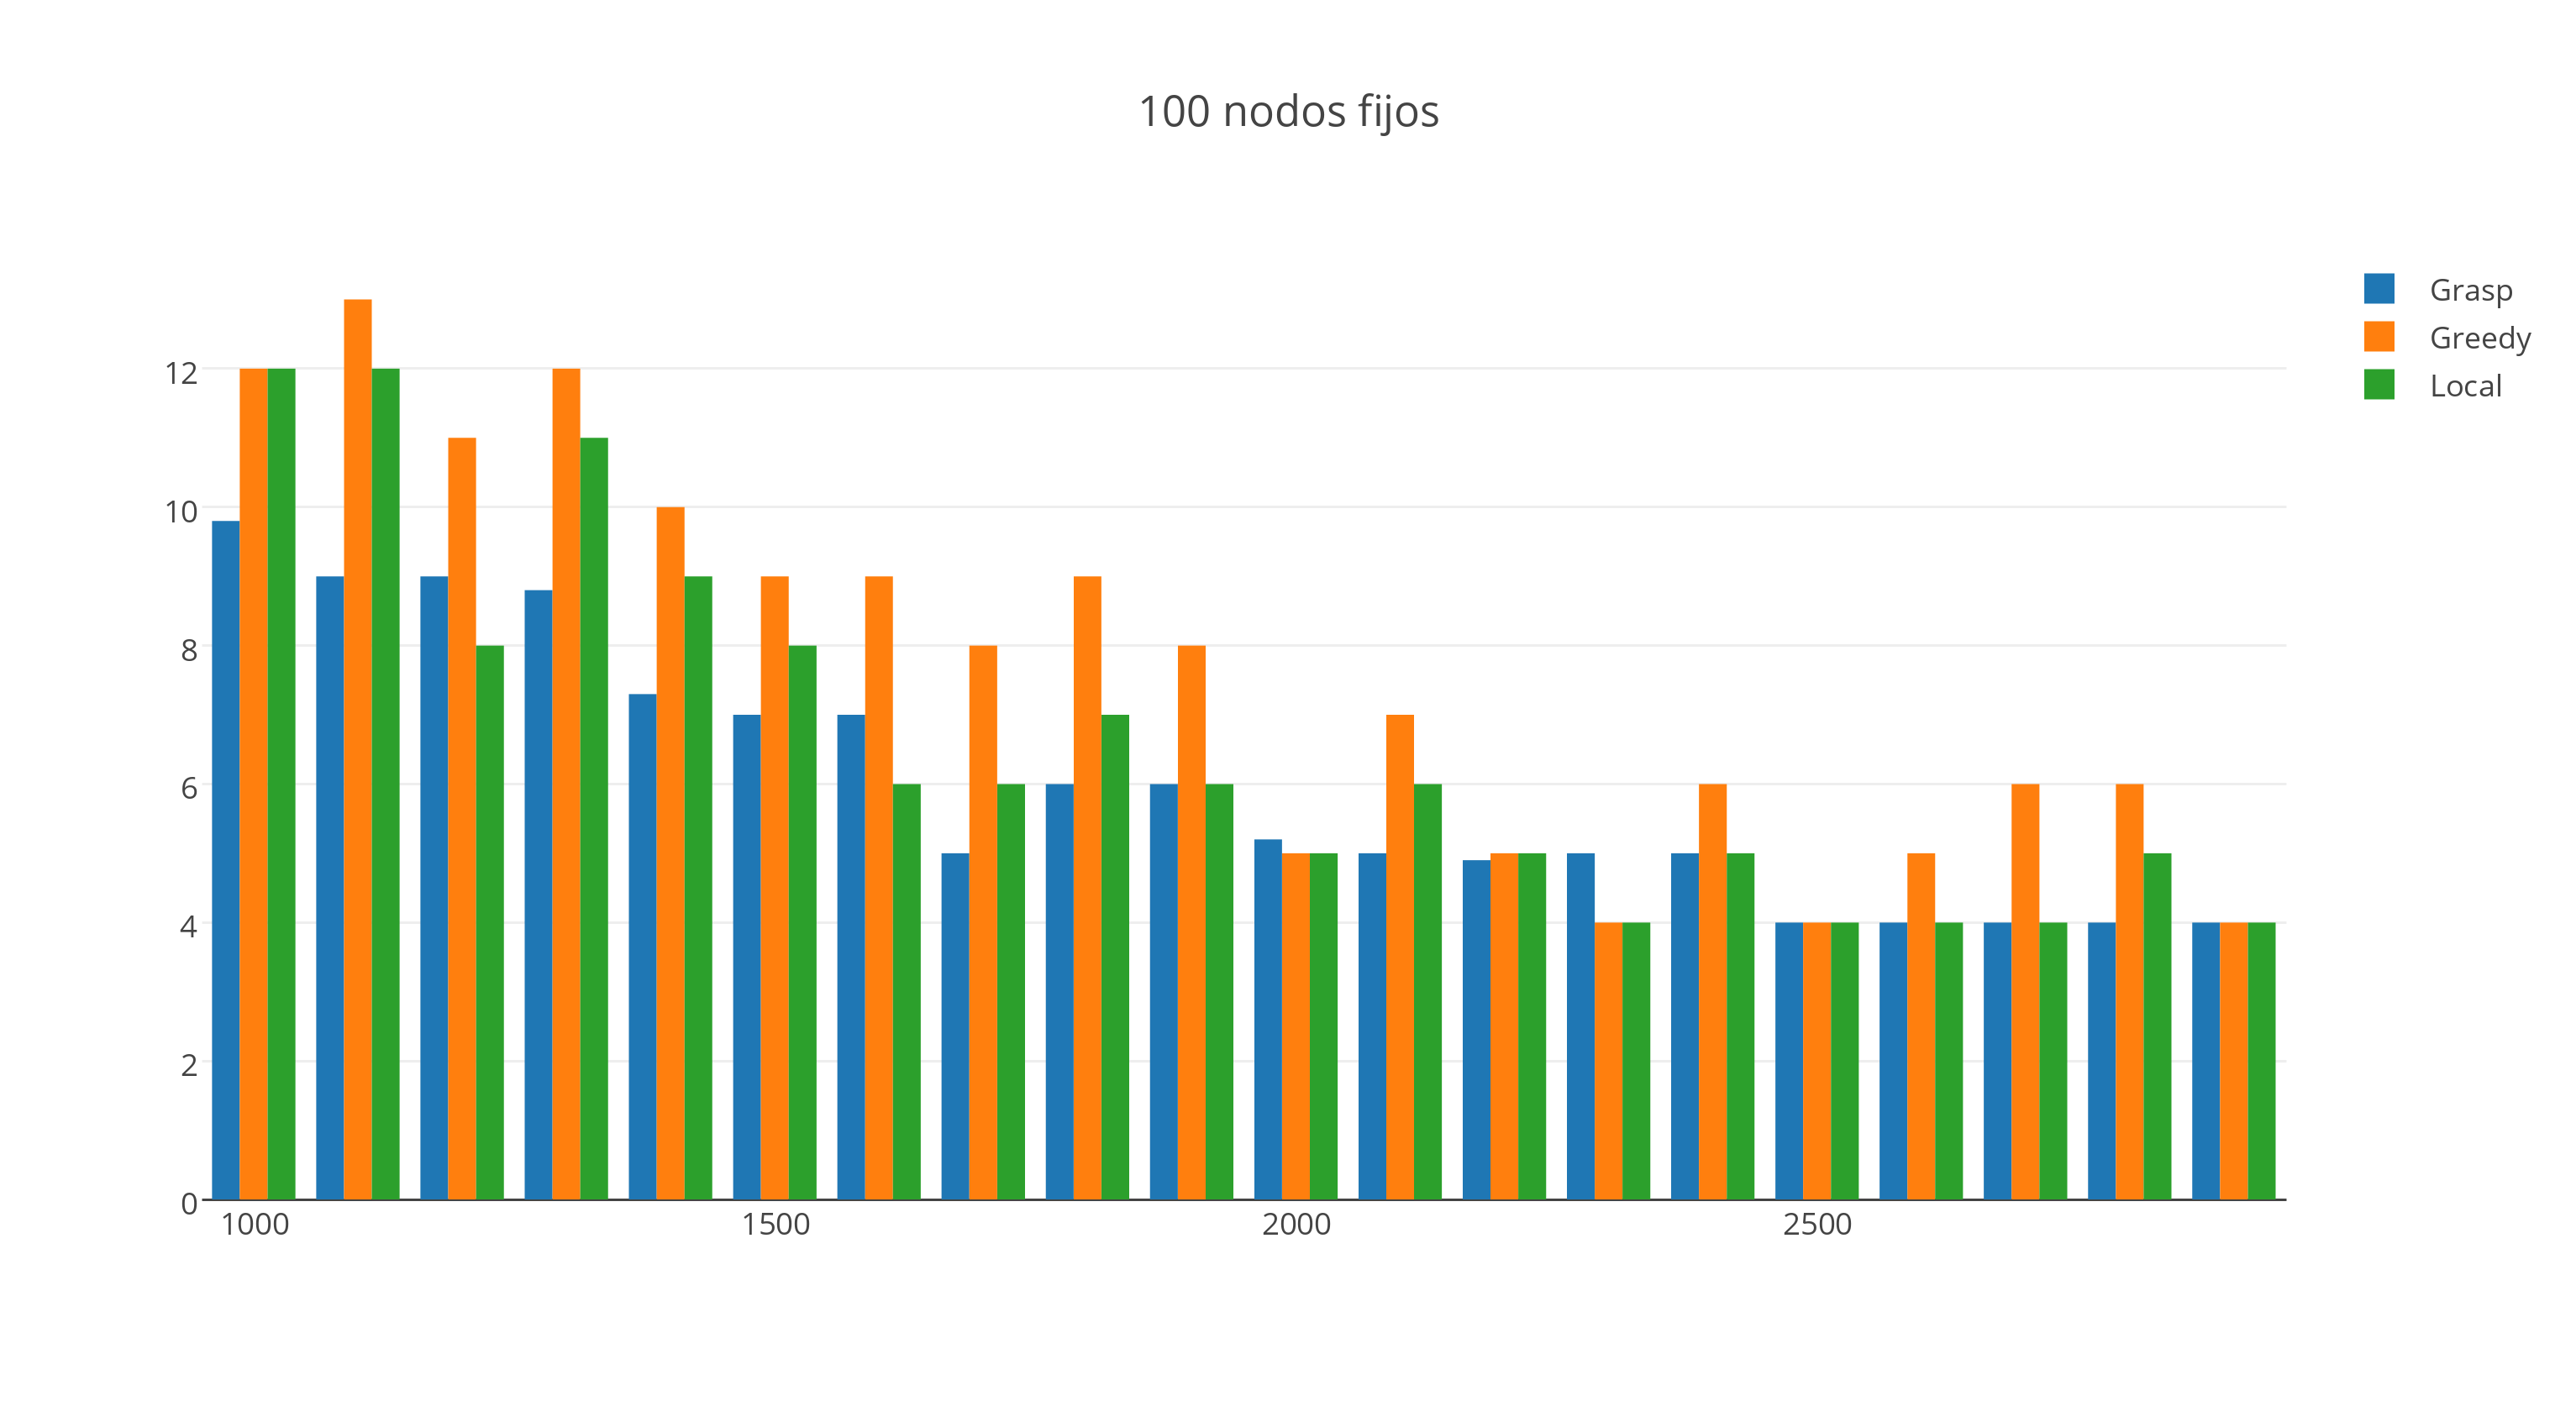
\includegraphics[scale=0.7]{imagenes/6/100NodosFijos.png}
% 	\caption{}
%	\label{}
   \end{center}
 \end{figure}
 
  \begin{figure}[h!]
   \begin{center}
 	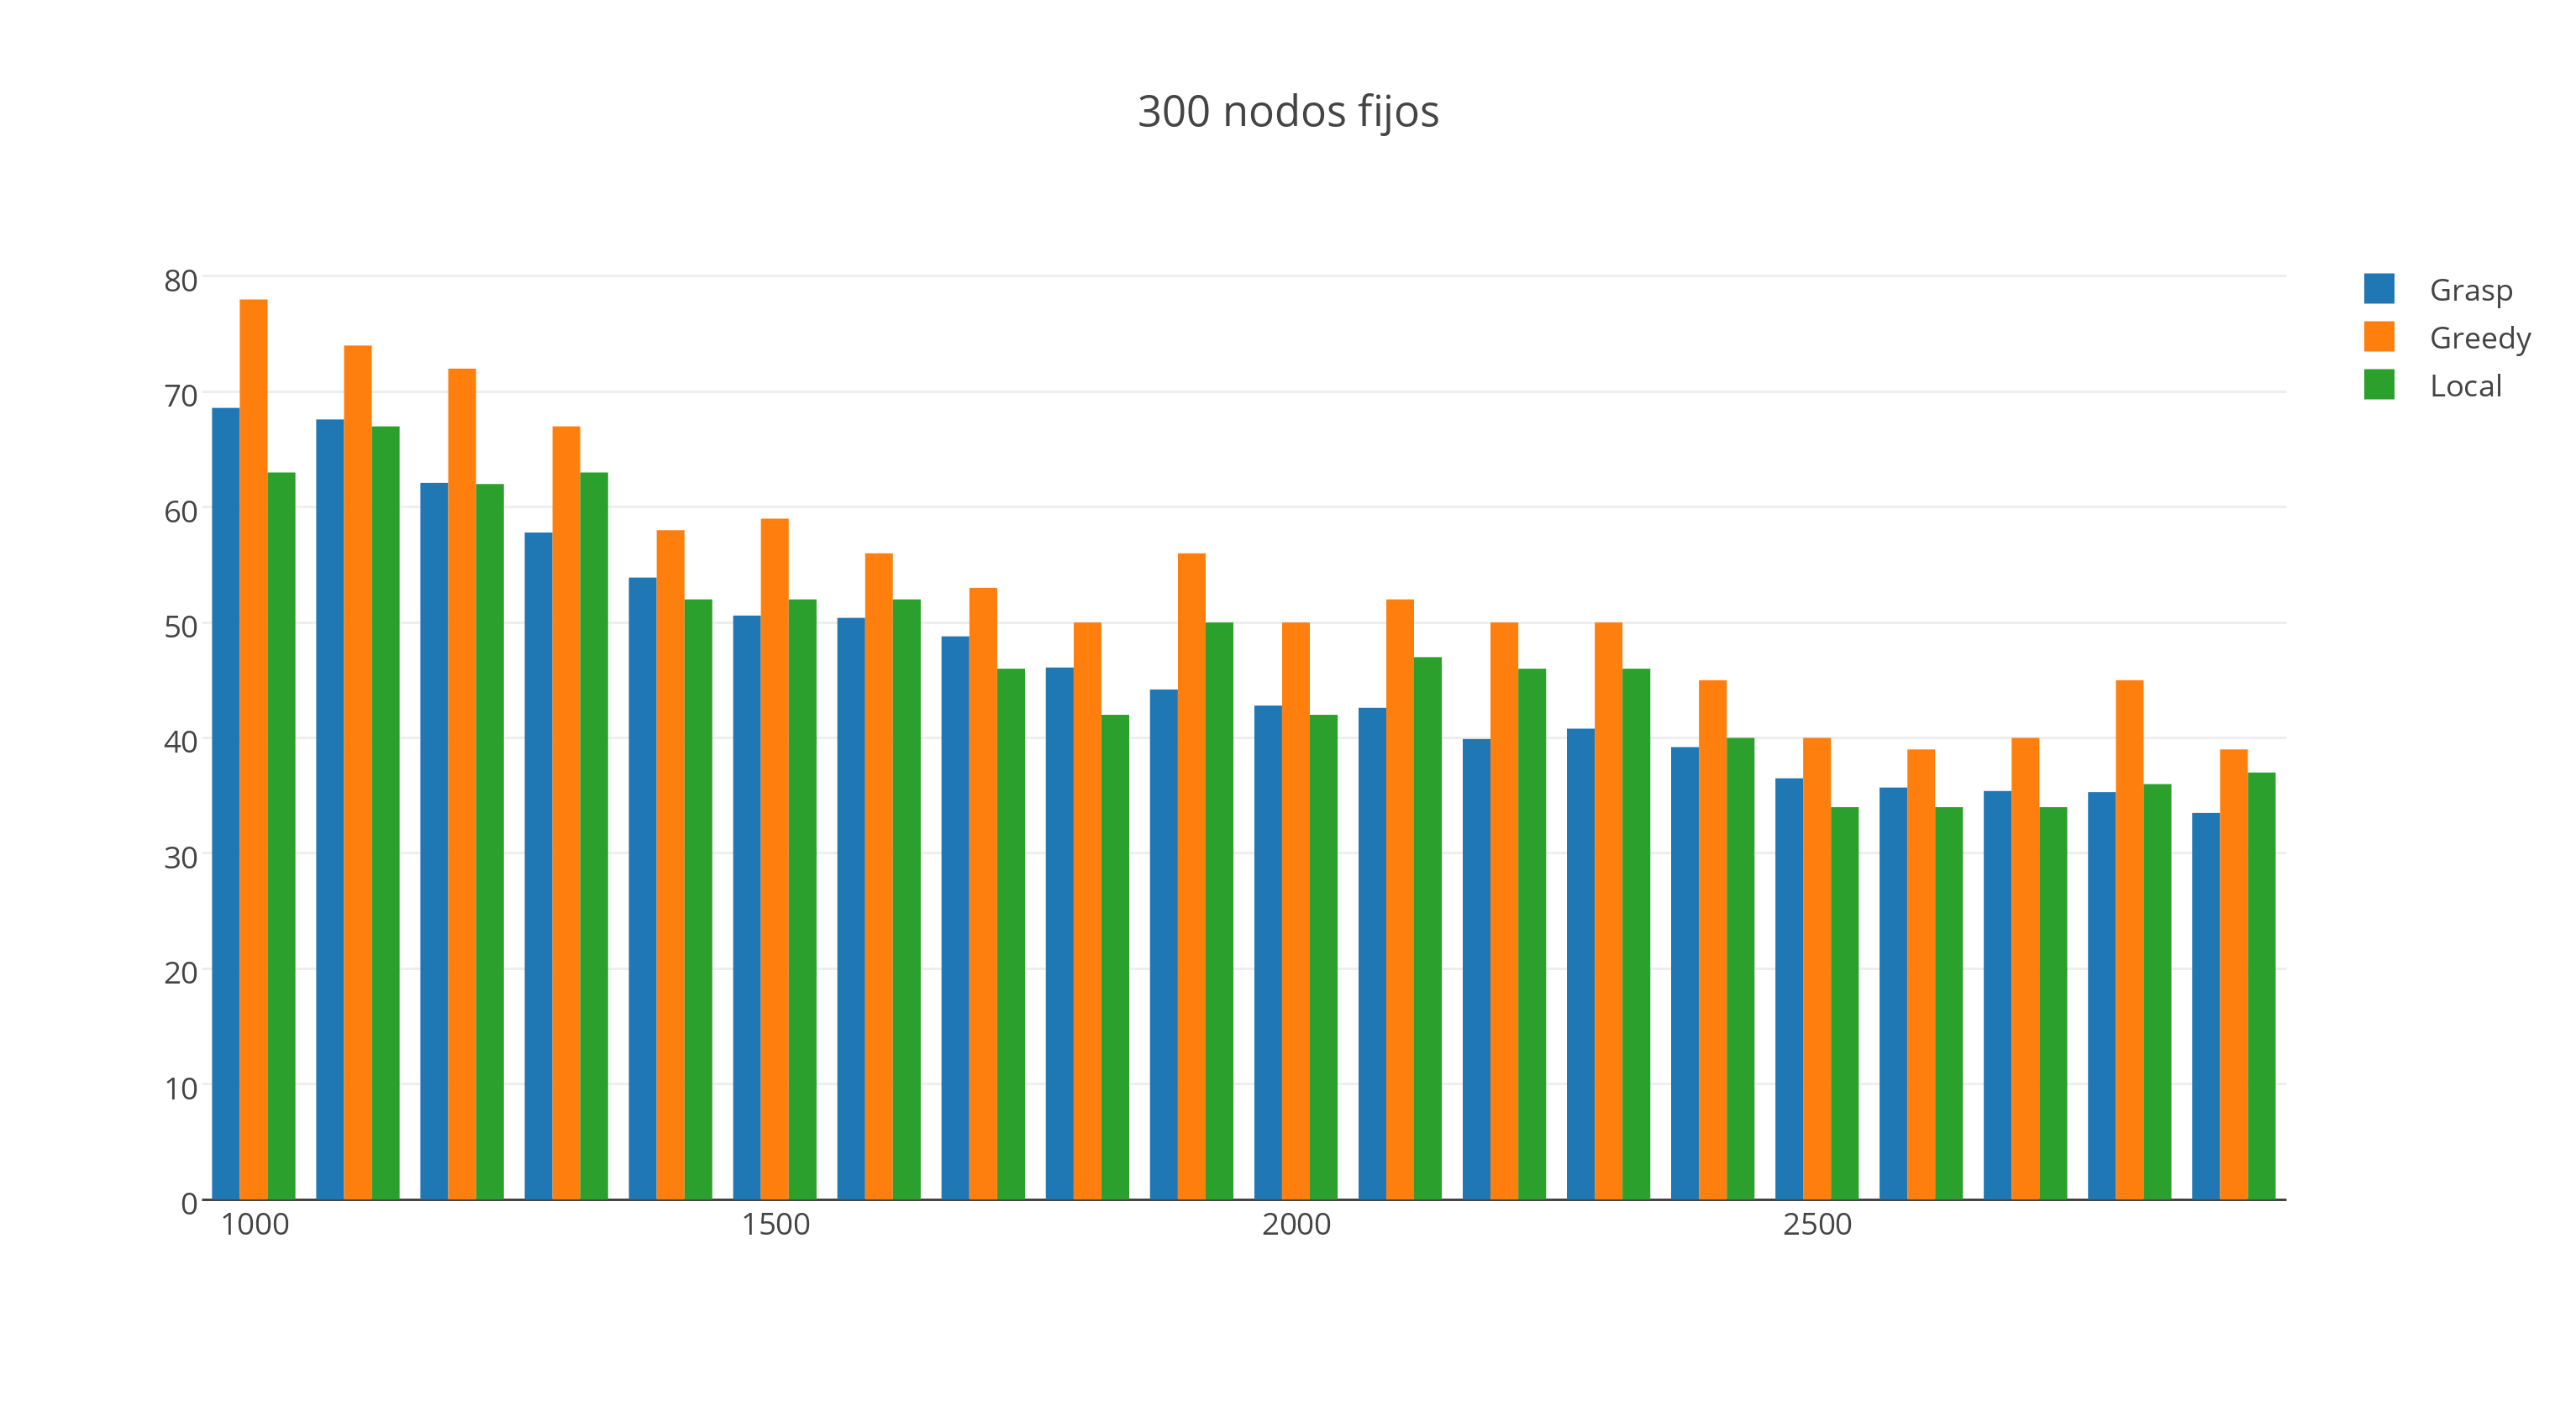
\includegraphics[scale=0.7]{imagenes/6/300NodosFijos.png}
% 	\caption{}
%	\label{}
   \end{center}
 \end{figure}
 
  \begin{figure}[h!]
   \begin{center}
 	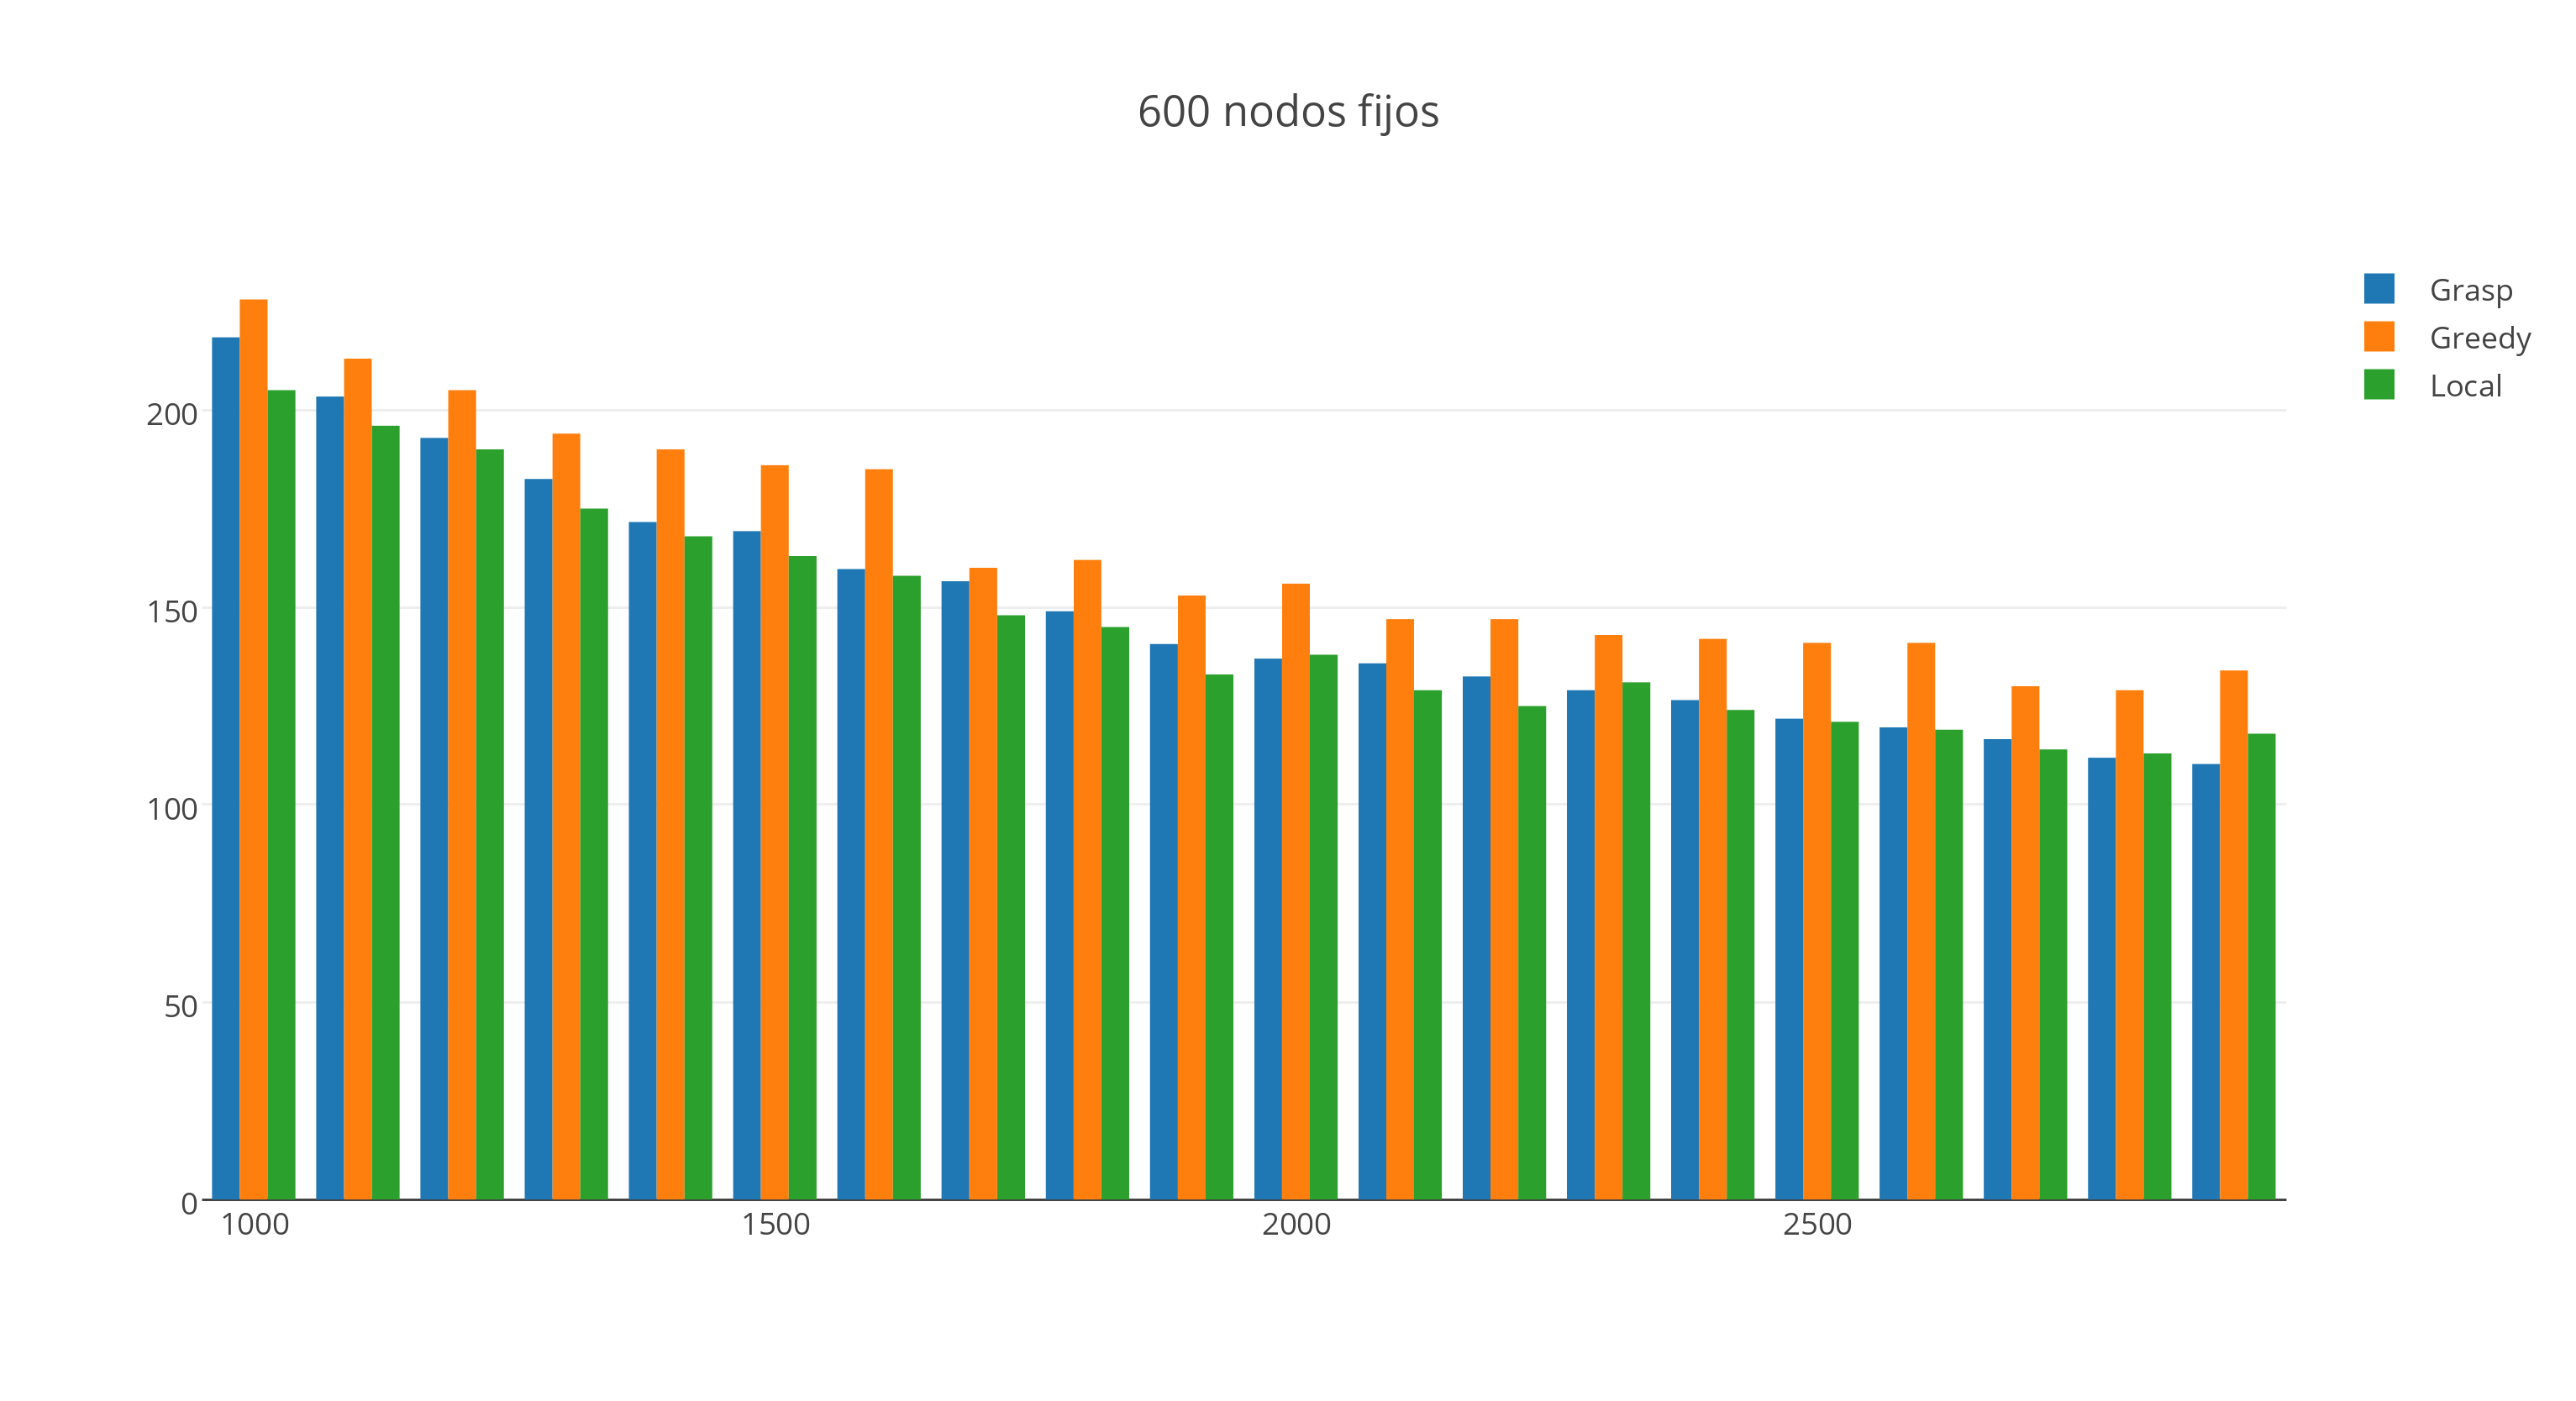
\includegraphics[scale=0.7]{imagenes/6/600NodosFijos.png}
% 	\caption{}
%	\label{}
   \end{center}
 \end{figure}
 
  \begin{figure}[h!]
   \begin{center}
 	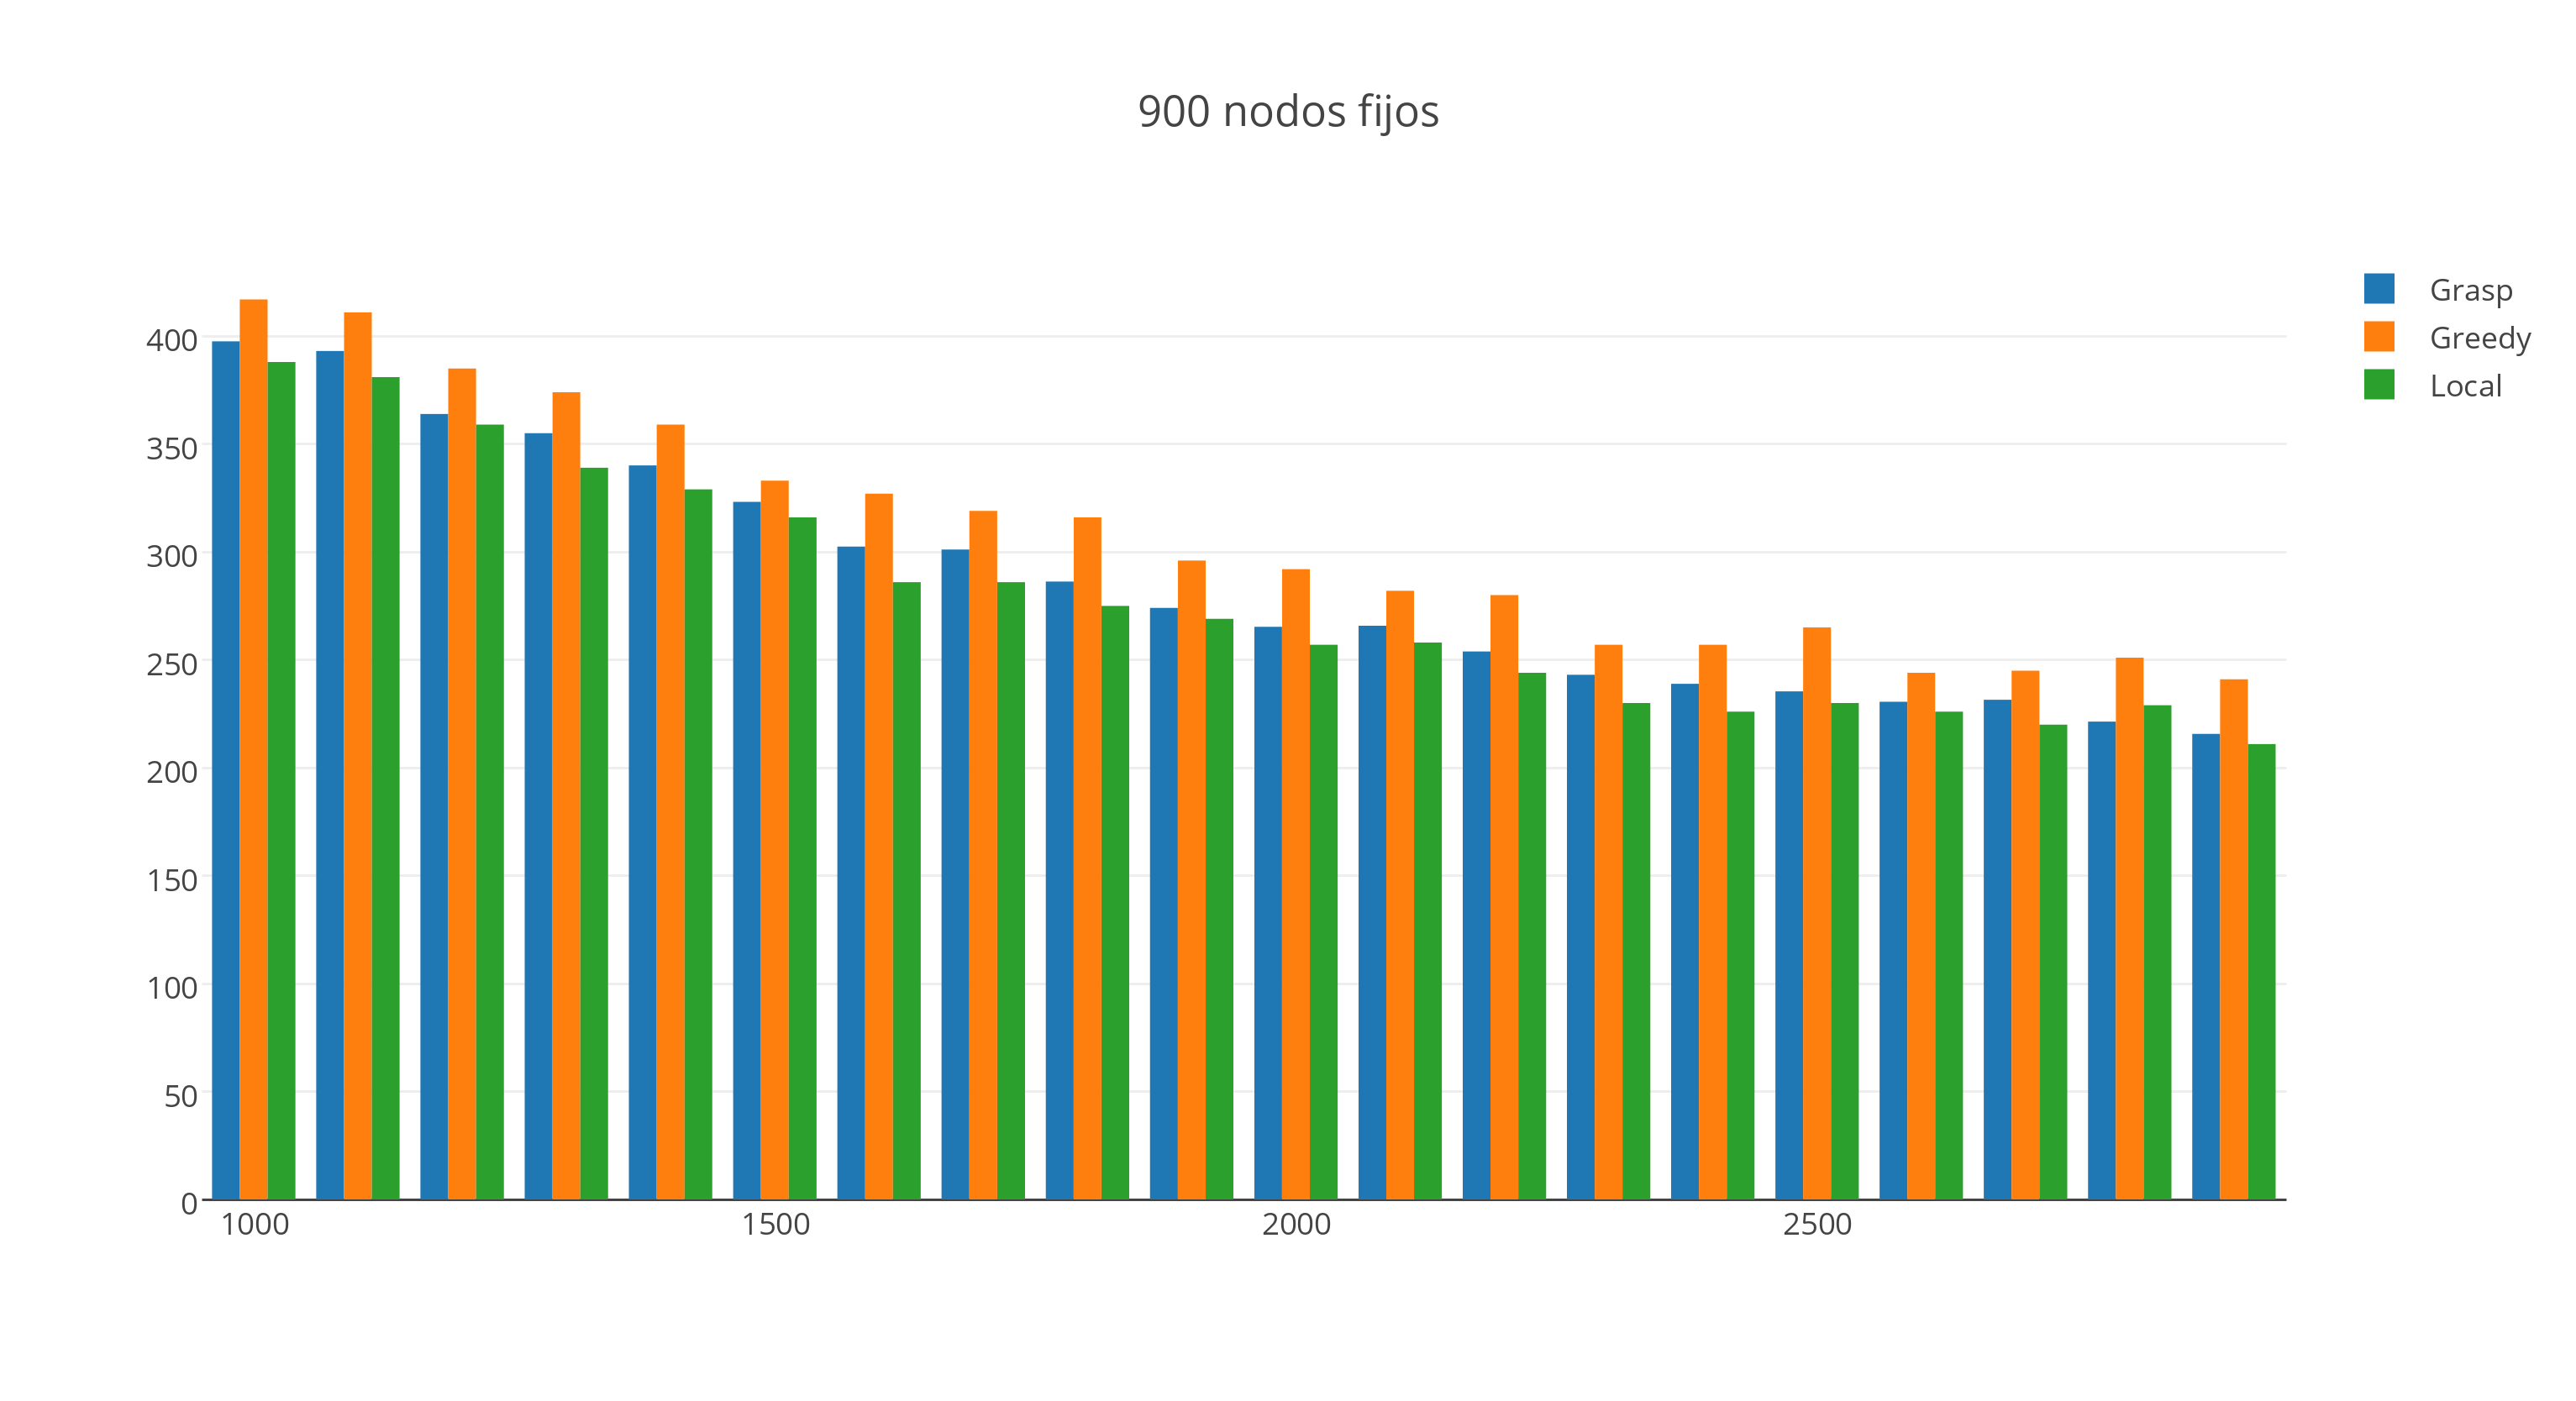
\includegraphics[scale=0.7]{imagenes/6/900NodosFijos.png}
% 	\caption{}
%	\label{}
   \end{center}
 \end{figure}
 
Analizando estos gr\'aficos, podemos ver r\'apidamente que el algoritmo Greedy nos devuelve en todos los casos una soluci\'on peor que los otros dos, ya que utiliza mayor cantidad de nodos.\\
Por otra parte, se puede ver cierta ventaja del Grasp para los casos m\'as chicos (100, 300 nodos), pero para los casos grandes (600, 900 nodos), se ve que el Local es mejor en casi todos los casos.\\

No podemos distinguir claramente cu\'al es la mejor opci\'on entre estos dos, ya que los valores son bastante cambiantes a lo largo de los 4 gr\'aficos, por lo que buscamos el promedio de nodos que utiliza
cada algoritmo. Los resultados fueron los siguientes:\\

\textcolor{red}{Tabla con promedios}

Estos promedios confirman los datos que se pod\'ian apreciar en los gr\'aficos, es decir, que el Greedy utiliza siempre mayor cantidad de nodos que los otros, que Grasp es mejor en los casos chicos y
que a medida que crece la cantidad de nodos, es preferible el Local.\\

\subsubsection{Ejes Fijos}
Para continuar, realizamos los mismos tests, pero manteniendo los ejes fijos y variando la cantidad de nodos. Los tests realizados fueron con ejes fijos desde 0 hasta 1000 y para cada instancia,
los nodos var\'ian de 50 a 1000.\\

Mostraremos los resultados obtenidos con 300, 600 y 900 ejes fijos:\\

  \begin{figure}[h!]
   \begin{center}
 	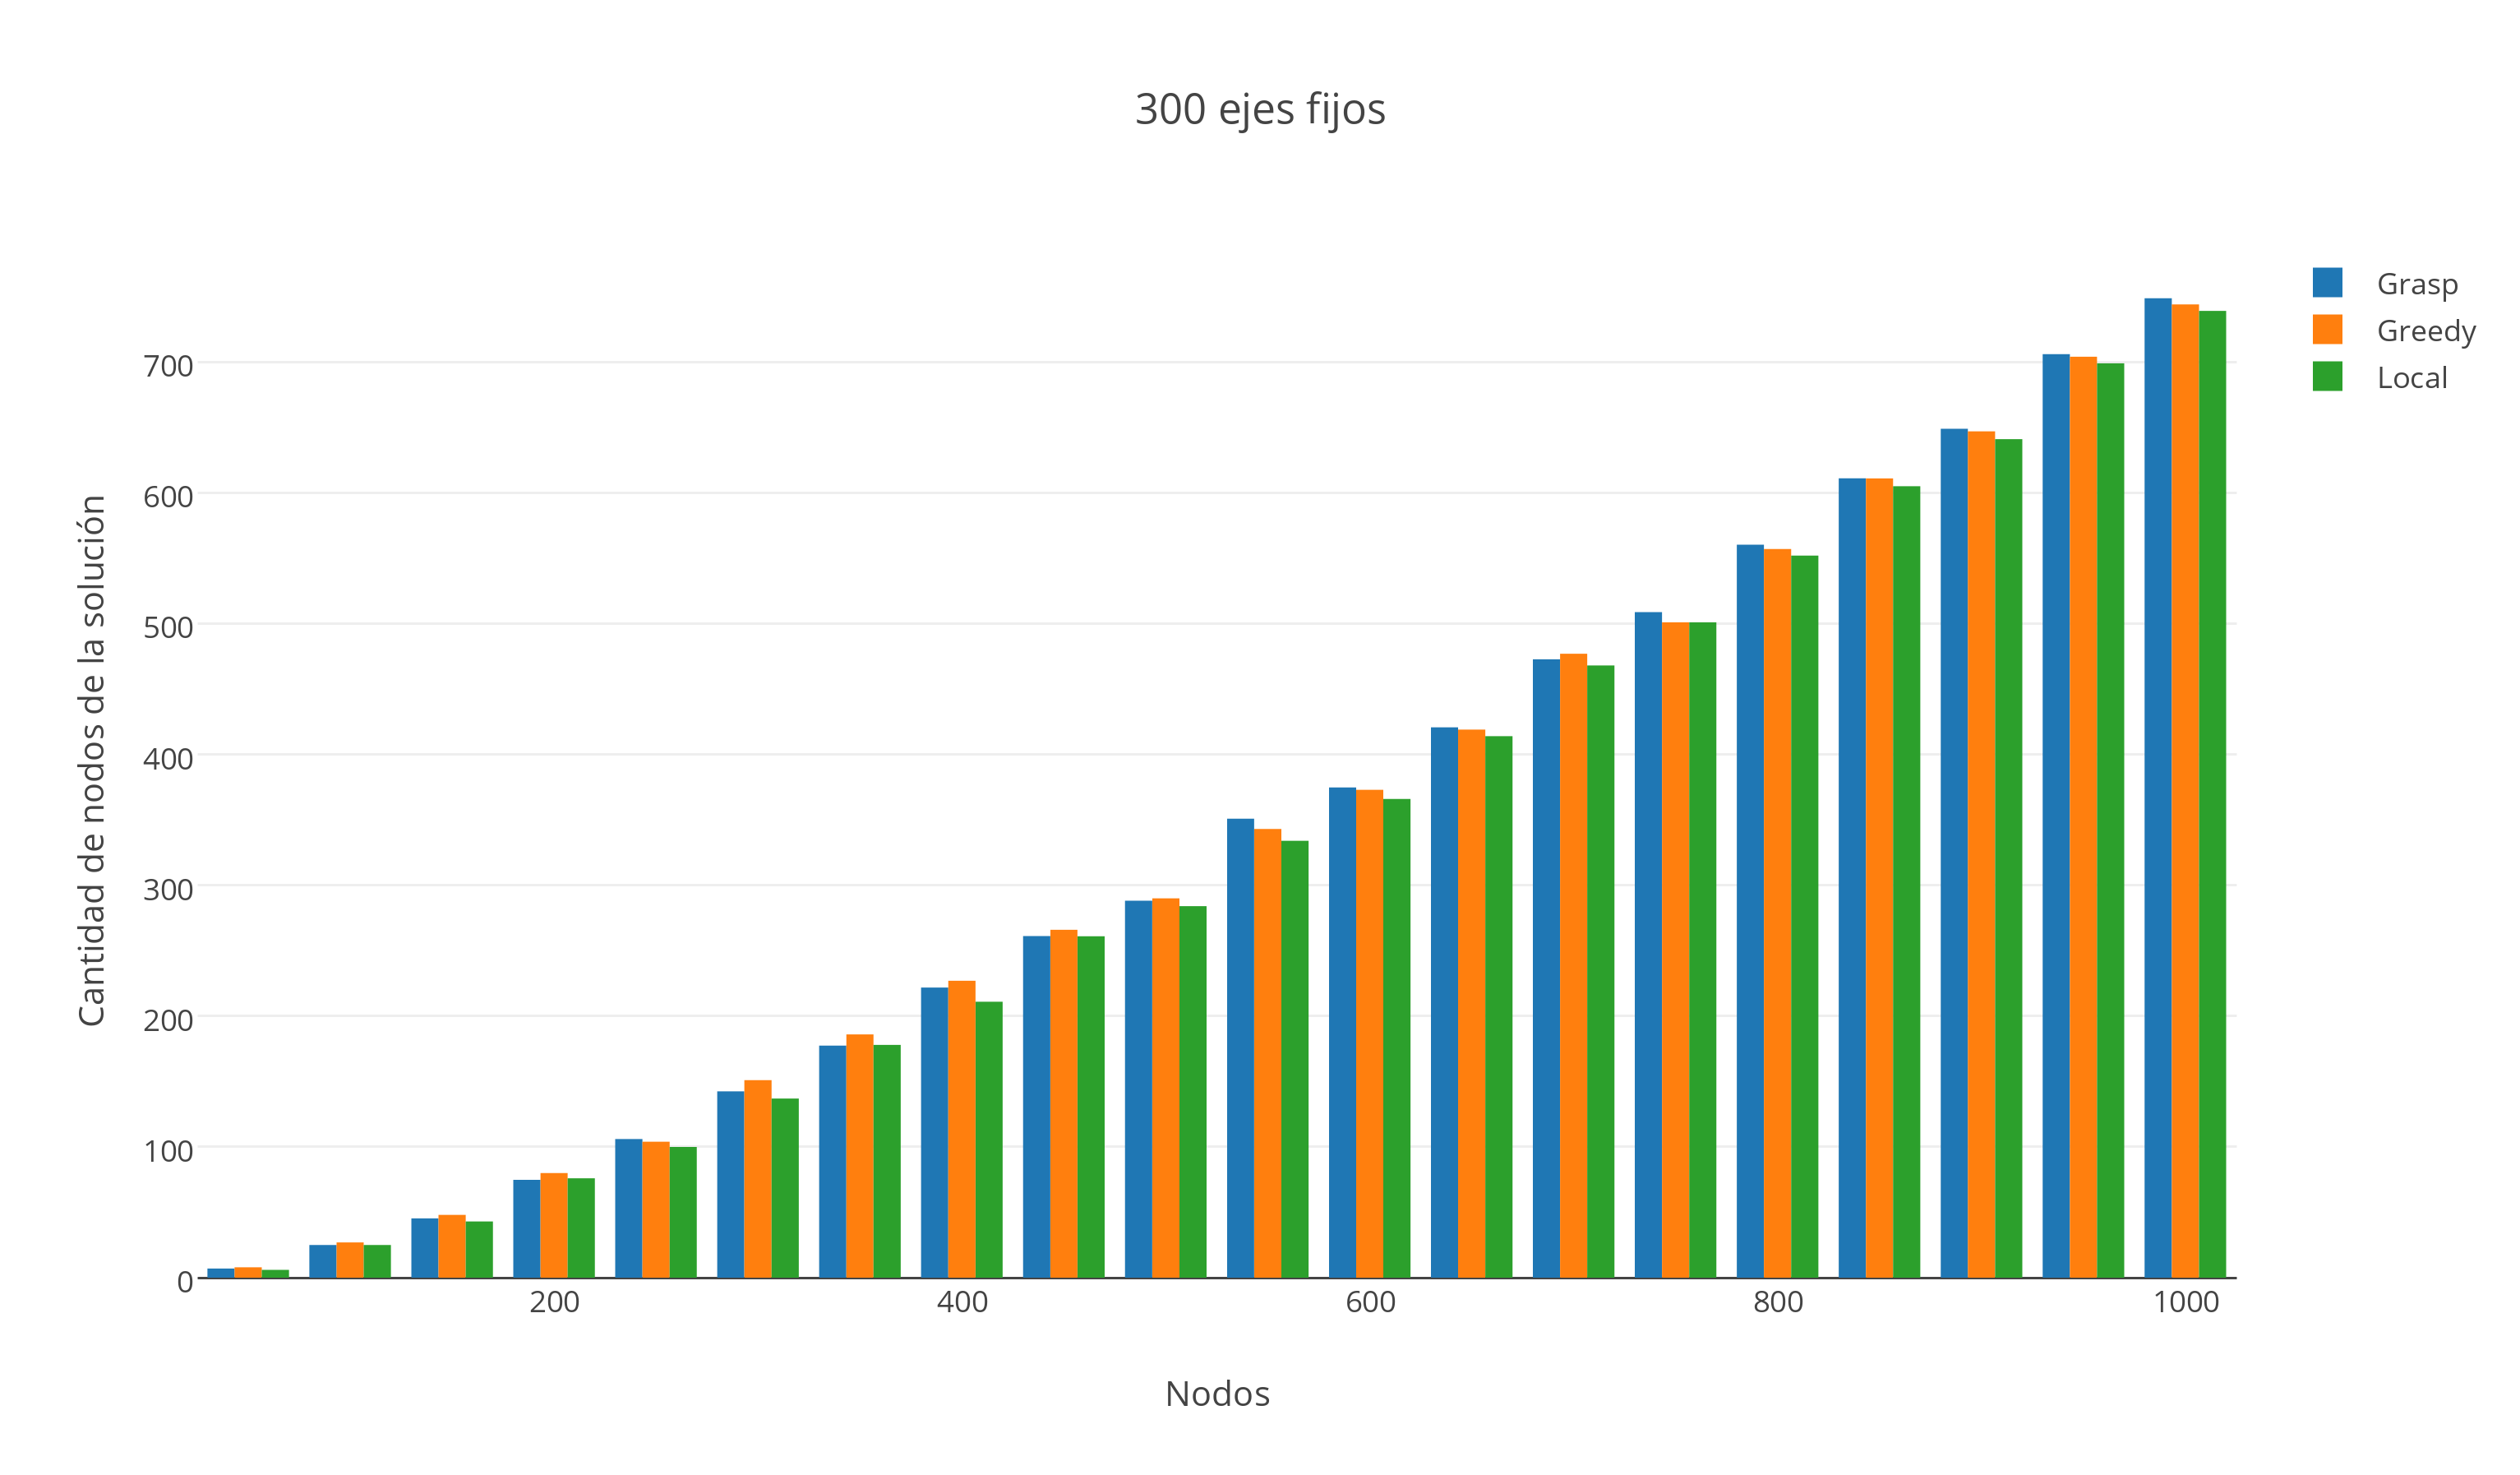
\includegraphics[scale=0.7]{imagenes/6/300EjesFijos.png}
% 	\caption{}
%	\label{}
   \end{center}
 \end{figure}
 
   \begin{figure}[h!]
   \begin{center}
 	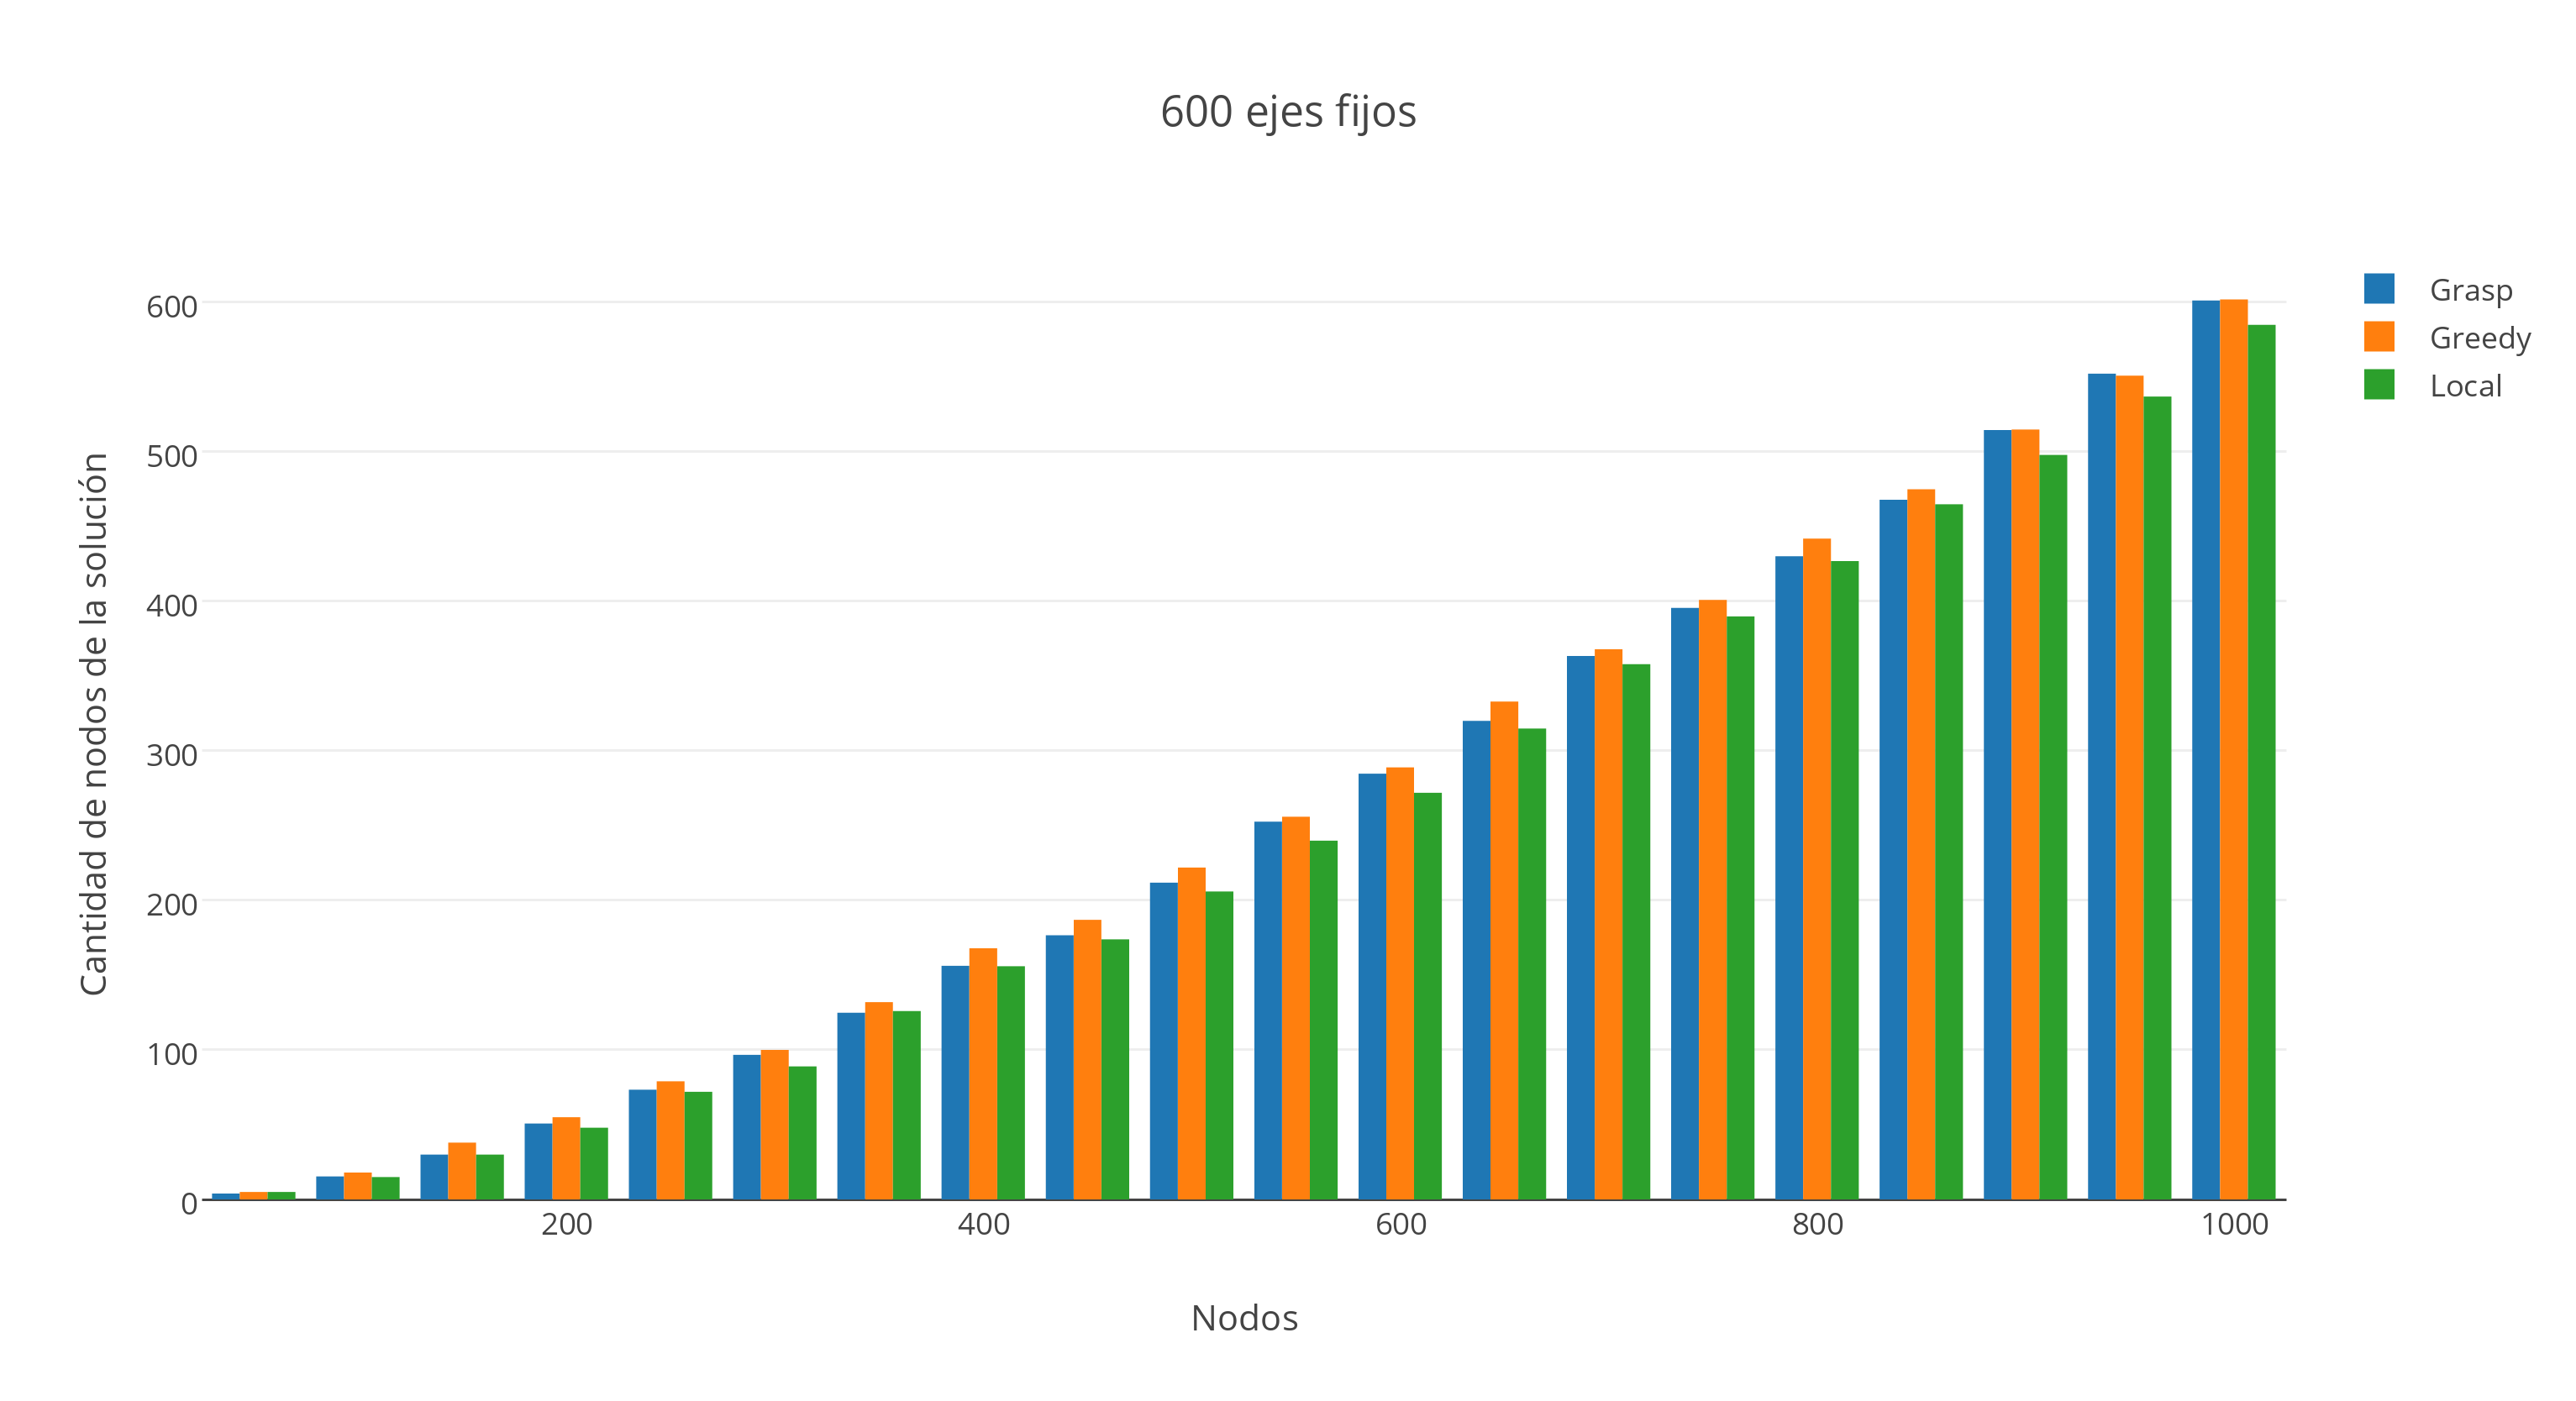
\includegraphics[scale=0.7]{imagenes/6/600EjesFijos.png}
% 	\caption{}
%	\label{}
   \end{center}
 \end{figure}

   \begin{figure}[h!]
   \begin{center}
 	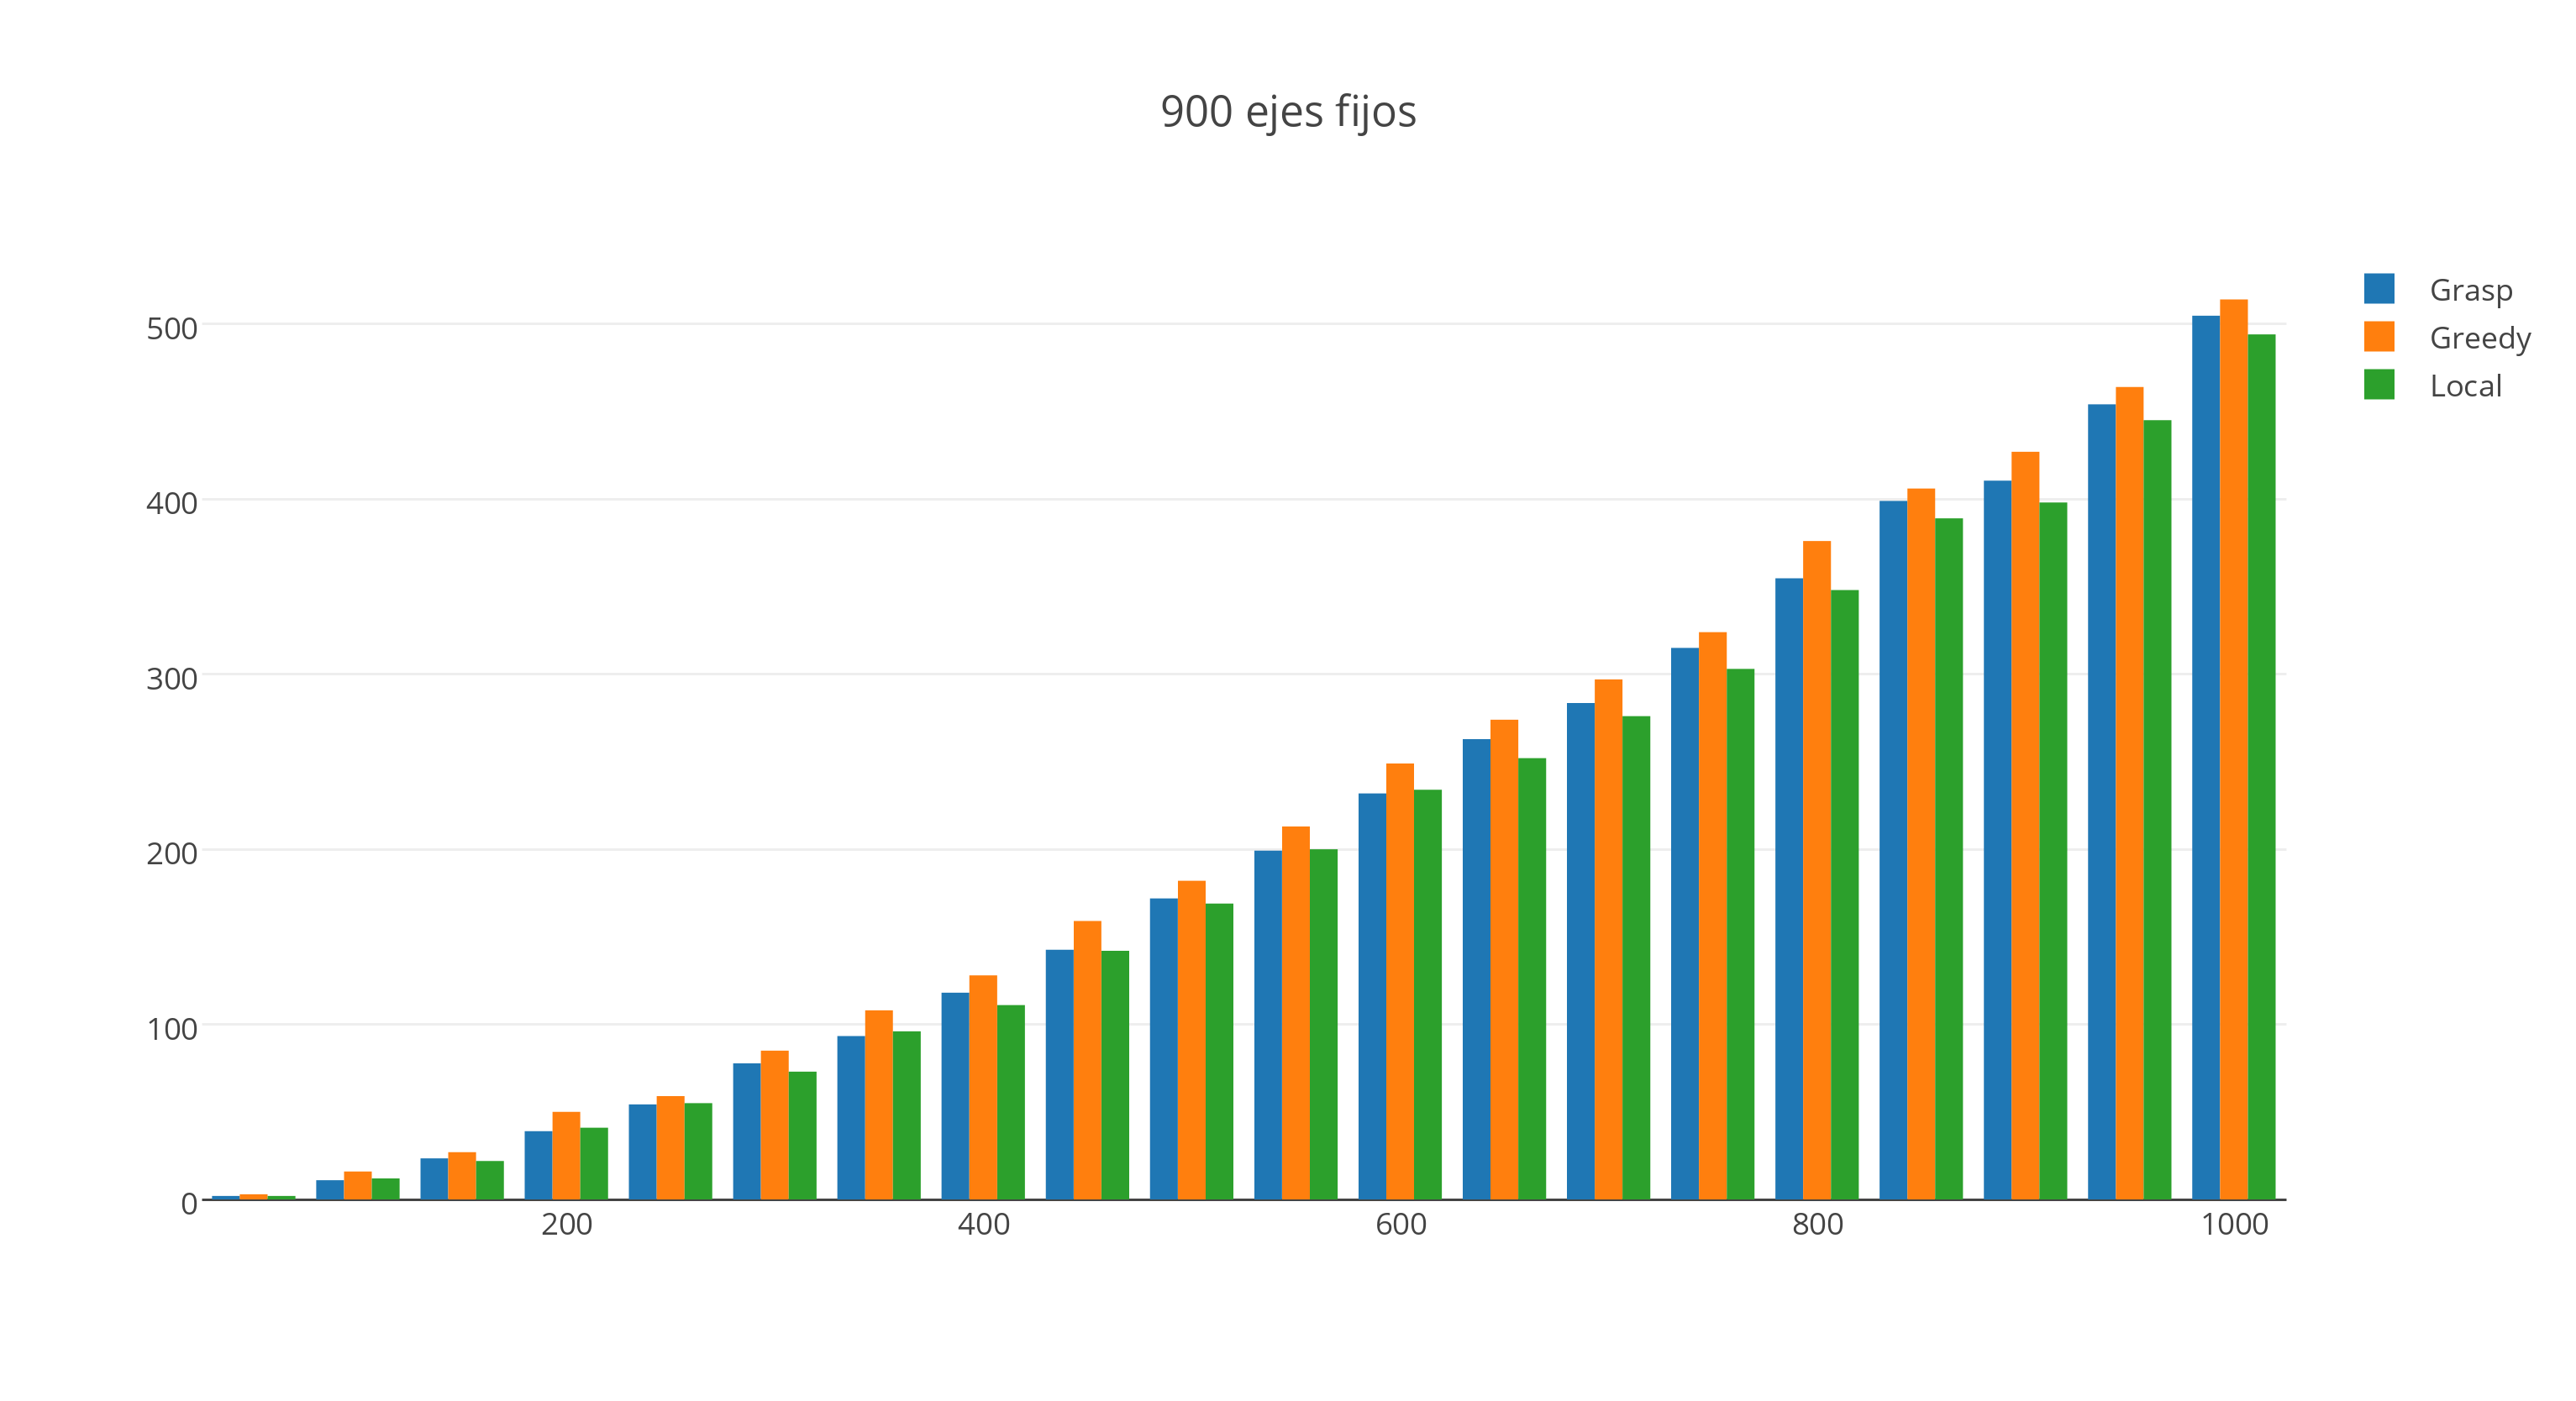
\includegraphics[scale=0.7]{imagenes/6/900EjesFijos.png}
% 	\caption{}
%	\label{}
   \end{center}
 \end{figure}
 
A primera vista, se puede ver que para casi todas las instancias el algoritmo de B\'usqueda Local es el que menos nodos utiliza en su soluci\'on. 
En cuanto al Greedy y el Grasp, las diferencias son chicas y alternadas con 300 ejes, pero con 600 y 900 ejes, Greedy aparenta ser el peor.\\

Para corroborar estos datos, tomamos nuevamente el promedio de todas las soluciones:\\

\textcolor{red}{Tabla con promedios}

Como preve\'iamos, estos promedios confirman nuestro an\'alisis.